\Wgstar\ is one of the critical backgrounds that we need to control
in order to have a reliable signal extraction. \WgstarMM\ process is
simulated using a dedicated Madgraph Monte Carlo generator and
cross-checked on data by explicitly reconstructing tri-lepton events
containing both muons from the virtual photon.
% (Section~\ref{sec:bkg_wgammastar}). 
For \WgstarEE\ process it is not
possible to perform a similar study on data due to large
backgrounds. Here we describe an alternative method for
estimation of the \WgstarEE\ contribution in data.

\Wgstar\ and \Zgstar\ processes are essentially identical with
respect to the internal conversion. We can compare a relative rate of
$\ell\ell\mu$ and $\ell\ell e$ by fit the tri-lepton mass
distribution, which will pick at the Z-boson mass for
asymmetric \ZgstarMM\ and \ZgstarEE\ events. Since events with the
asymmetric internal conversion represent majority of \Wgstar\ events
that enter the \hww\ analysis, we can test how well Monte Carlo
predicts the relative contribution of $\gamma^*\to\mu\mu$ and
$\gamma^*\to ee$ processes.

We select dilepton events using the nominal lepton identification
requirements and invariant mass less than 75~\GeV{}. We also require a
third lepton passing the same lepton identification requirements. The
tri-lepton mass distributions in data are shown on
Figure~\ref{fig:appendix_zgstar_data}. Performing the
maximum-likelihood fit with the Crystal ball signal shape and the 2nd
order Chebyshev polynomial for background, we find
$N_{\ell\ell\mu}=404.0\pm27.9$ and $N_{\ell\ell
e}=430.7\pm25.5$. 

$N_{\ell\ell e}$ contains $Z\to\ell\ell\gamma$ events with the photon
conversion in the detector material that needs to be properly
estimated. We perform the same maximum-likelihood fit on \dyll\ Monte
Carlo events and use the event yield from the fit as an estimation of
the real conversion contribution to $N_{\ell\ell e}$. We find the
event yield to be $86.3\pm9.5$. Taking into account efficiency and
integrated luminosity we get $N_{\mathrm{conv}}=175\pm19$ as an
estimation of the real conversion to $N_{\ell\ell e}$.

\begin{equation}
    R_Z = \frac{N_{\ell\ell\mu}}{N_{\ell\ell e}} = 1.58\pm0.22
\end{equation}

Forming a similar ration using \Wgstar\ Monte Carlo simulations we get:

\begin{equation}
    R_W = \frac{N_{\ell\mu}}{N_{\ell e}} = 1.81\pm0.06
\end{equation}

Given that $R_Z$ and $R_W$ are statistically consistent, it means
corrections applied to \WgstarMM\ Monte Carlo simulated events can be
used for \WgstarEE\ as well.

\begin{figure}[!hbtp]
\centering
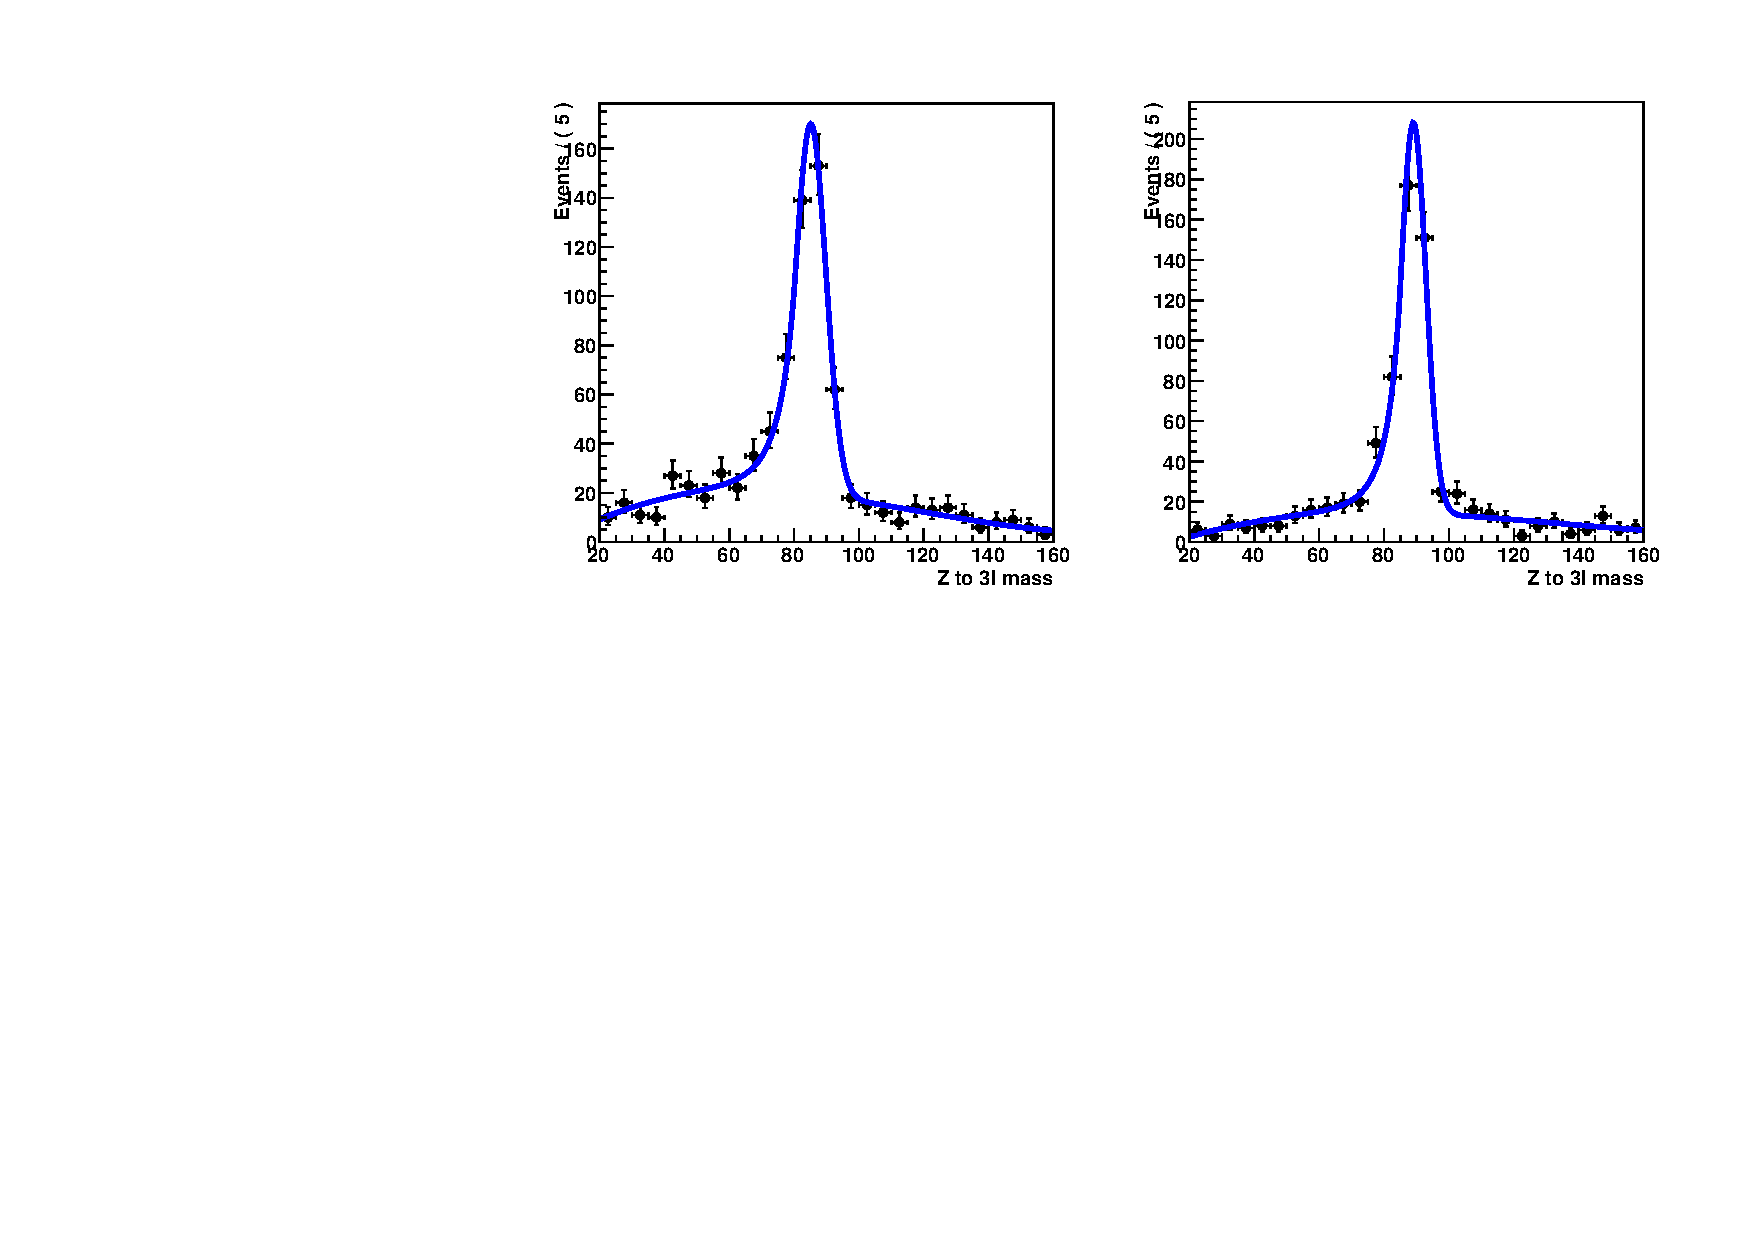
\includegraphics[width=.75\textwidth]{figures/appendix_zgstar_data.pdf}
\caption{Tri-lepton mass distribution for $\ell\ell\mu$ (left) and 
$\ell\ell e$ (right) for 19.3~\ifb\ of 8~\TeV\ data.}
\label{fig:appendix_zgstar_data}
\end{figure}

